\section{Model Component} \label{sc:model_component}
Based on the analysis of the problem domain, through the class diagram, event table and state charts. It it possible to create an updated model of the problem domain. 
\par
This is done by specifying the model component mentioned in section \ref{sc:component_architecture}. The result is an updated class diagram, that contains attributes and operations. 

% Tags og andre ting skal introduceres inden dette afsnit
\begin{figure}[H]
    \centering
    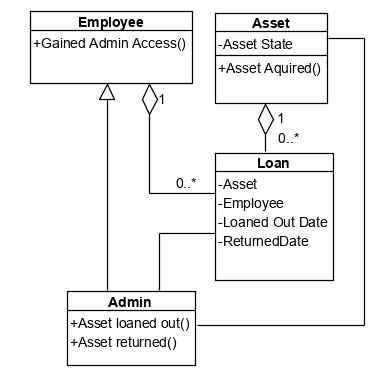
\includegraphics[width=0.8\textwidth]{figures/Model_ComponentV2.PNG}
    \caption{Diagram of the model component}
    \label{fig:ModelComponent}
\end{figure}

As illustrated in figure \ref{fig:ModelComponent} ...